\documentclass[12pt,a4paper]{article}
\title{%
  Øving 3 \\
  \large IELET1002 - Datateknikk \\
  }
\author{Gunnar Myhre, BIELEKTRO}

\usepackage[utf8]{inputenc}
\usepackage[norsk]{babel}
\usepackage[siunitx]{circuitikz}
\usepackage{karnaugh-map}
\graphicspath{ {./images} }

\newcommand{\N}{\overline}

\setlength\parindent{0pt}

\begin{document}
  \maketitle
    \section{Oppgåve 1}
      Setter opp funksjonstabell for 4-bit gray-kode
      \begin{center}
        \begin{tabular}{ |c|c|c|c|c| c|c|c|c|c|c|c| }
          \hline
          Indeks & $a_3a_2a_1a_0$ & $g_3g_2g_1g_0$ \\
          \hline
          0  &  0000 & 0000 \\
          \hline
          1  &  0001 & 0001 \\
          \hline
          2  &  0010 & 0011 \\
          \hline
          3  &  0011 & 0010 \\
          \hline
          4  &  0100 & 0110 \\
          \hline
          5  &  0101 & 0111 \\
          \hline
          6  &  0110 & 0101 \\
          \hline
          7  &  0111 & 0100 \\
          \hline
          8  &  1000 & 1100 \\
          \hline
          9  &  1001 & 1101 \\
          \hline
          10 &  1010 & 1111 \\
          \hline
          11 &  1011 & 1110 \\
          \hline
          12 &  1100 & 1010 \\
          \hline
          13 &  1101 & 1011 \\
          \hline
          14 &  1110 & 1001 \\
          \hline
          15 &  1111 & 1000 \\
          \hline
        \end{tabular}
      \end{center}

      Frå dette finner vi sum av standardprodukt
      \begin{itemize}
        \item $g_3= \Sigma(8,9,10,11,12,13,14,15)$
        \item $g_2= \Sigma(4,5,6,7,8,9,10,11)$
        \item $g_1= \Sigma(2,3,4,5,10,11,12,13)$
        \item $g_0= \Sigma(1,2,5,6,9,10,13,14)$
      \end{itemize}

      Teikner opp Karnaugh-diagram
      \begin{center}
        \begin{karnaugh-map}[4][4][1][$a_1a_0$][$a_3a_2$]
          \minterms{8,9,10,11,12,13,14,15}
          \maxterms{0,1,2,3,4,5,6,7}
          \implicant{12}{10}
        \end{karnaugh-map}
      \end{center}
      $g_3 = a_3$

      \begin{center}
        \begin{karnaugh-map}[4][4][1][$a_1a_0$][$a_3a_2$]
          \minterms{4,5,6,7,8,9,10,11}
          \maxterms{0,1,2,3,12,13,14,15}
          \implicant{8}{10}
          \implicant{4}{6}
        \end{karnaugh-map}
      \end{center}
      $g_2 = \N{a_3}a_2+a_3\N{a_2}$

      \begin{center}
        \begin{karnaugh-map}[4][4][1][$a_1a_0$][$a_3a_2$]
          \minterms{2,3,4,5,10,11,12,13}
          \maxterms{0,1,6,7,8,9,14,15}
          \implicant{4}{13}
          \implicantedge{3}{2}{11}{10}
        \end{karnaugh-map}
      \end{center}
      $g_1 = \N{a_2}a_1+a_2\N{a_1}$

      \begin{center}
        \begin{karnaugh-map}[4][4][1][$a_1a_0$][$a_3a_2$]
          \minterms{1,2,5,6,9,10,13,14}
          \maxterms{0,3,4,7,8,11,12,15}
          \implicant{1}{9}
          \implicant{2}{10}
        \end{karnaugh-map}
      \end{center}
      $g_2 = \N{a_1}a_0+a_1\N{a_0}$. Forenkler uttrykka vha. XOR sidan $\N{A}B+A\N{B}=A\oplus B$

      \begin{itemize}
        \item $g_3 = a_3$
        \item $g_2 = a_3\oplus a_2$
        \item $g_1 = a_2\oplus a_1$
        \item $g_0 = a_1\oplus a_0$
      \end{itemize}
      \begin{center}
        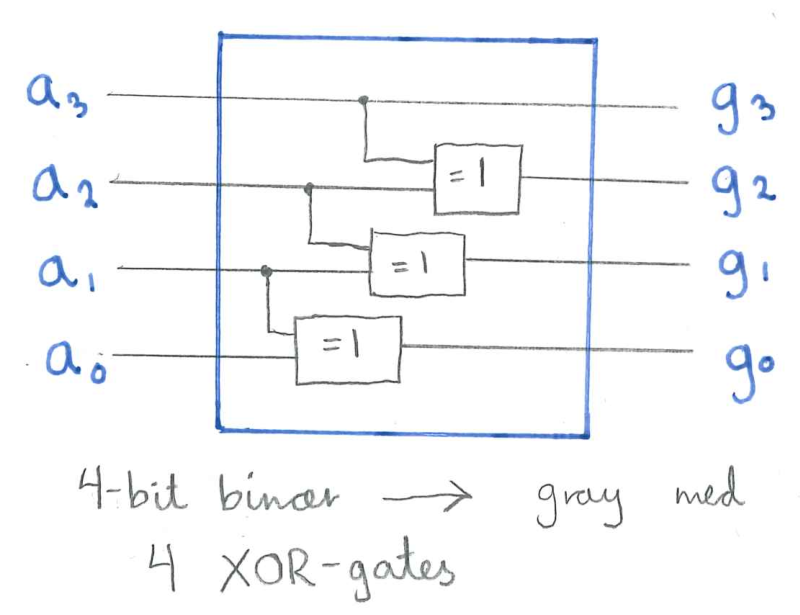
\includegraphics[width=83mm]{03_1}
      \end{center}

    \section{Oppgåve 2}
      \subsection{a)}
        Først setter vi opp funksjonstabell
        \begin{center}
          \begin{tabular}{ |c|c|c| }
            \hline
            $S_1$ & $S_0$ & $m_3m_2m_1m_0$ \\
            \hline
            0 & 0 & 0  0  0  1 \\
            \hline
            0 & 1 & 0  0  1  0 \\
            \hline
            1 & 0 & 0  1  0  0 \\
            \hline
            1 & 1 & 1  0  0  0 \\
            \hline
          \end{tabular}
        \end{center}

        uttrykka er gitt ved
        \begin{itemize}
          \item $m_0 = \bar{S_1}\bar{S_0}$
          \item $m_1 = \bar{S_1}S_0$
          \item $m_2 = S_1\bar{S_0}$
          \item $m_3 = S_1S_0$
        \end{itemize}

        vi kan teikne dette som eit logisk skjema vha. åtte AND-portar
        \begin{center}
          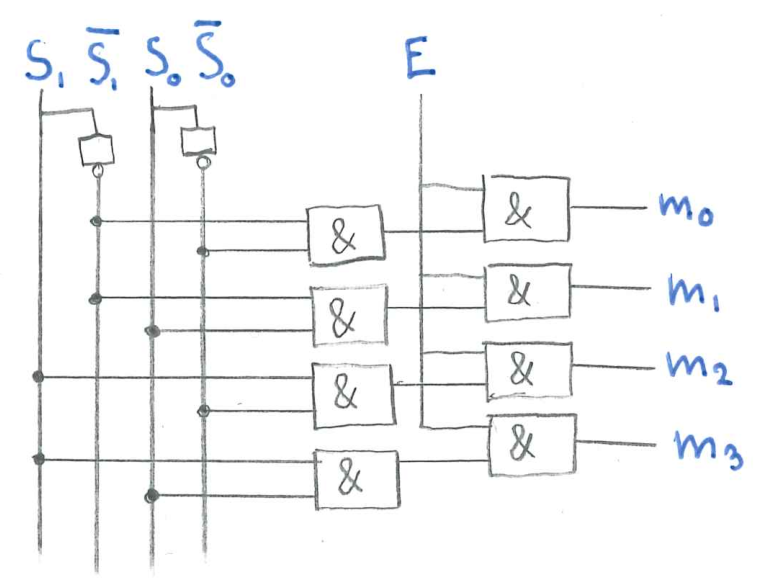
\includegraphics[width=83mm]{03_2a}
        \end{center}

      \subsection{b)}
        Funksjonen $F(x,y) = \Sigma(1,2)$ kan implementerast med ein XOR-port. Men dersom vi
        ønsker å bruke ein 2$\rightarrow$4-dekodar kan vi gjere slik som dette:

        \begin{center}
          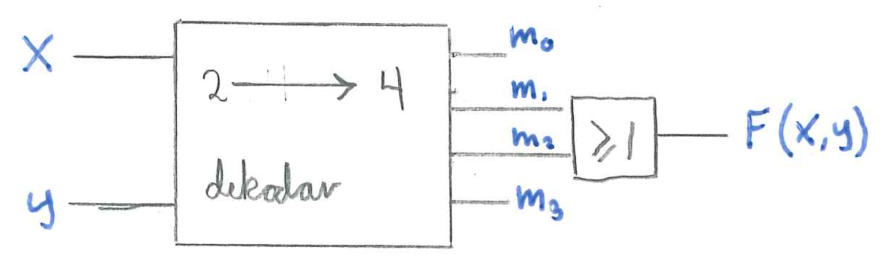
\includegraphics[width=83mm]{03_2b2}
        \end{center}
        Vi kan også implementere denne funksjonen med to NOT-portar, to AND-portar og éin OR-port
        \begin{center}
          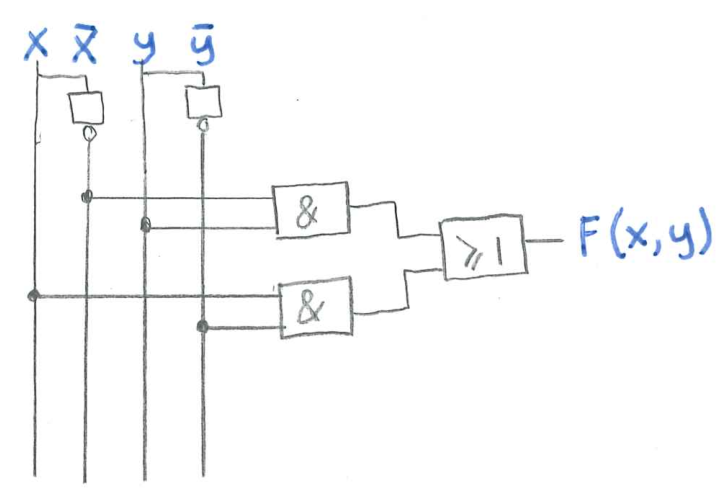
\includegraphics[width=83mm]{03_2b}
        \end{center}

    \section{Oppgåve 3}
      Antar at det her er snakk om fire databit og ikkje fire addressebit for multipleksaren.
      Då kan vi implementere den vha. ein 2$\rightarrow$4-dekodar slik som dette:

      \begin{center}
        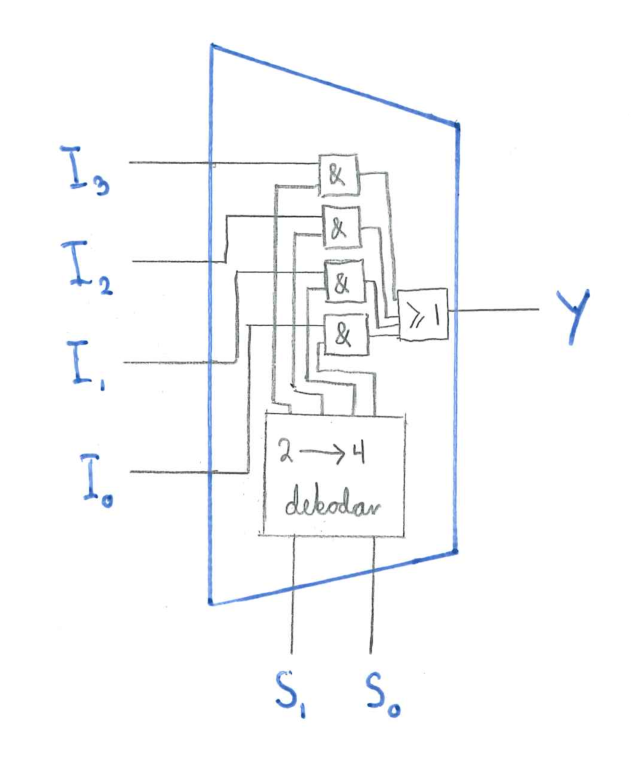
\includegraphics[width=83mm]{03_3}
      \end{center}
      Dekodaren som styrt av $S_1$ og $S_0$ velger kva for input $I$ som har moglegheit
      til å slippe igjennom til utgongen Y

    \section{Oppgåve 4}
      \subsection{a)}
        Setter først opp ufullstendig funksjonstabell for ein 4$\rightarrow$2-kodar
          \begin{center}
            \begin{tabular}{ |c|c|c| }
              \hline
              $I_0I_1I_2I_3$ & $S_1$ & $S_0$ \\
              \hline
              1000 & 0 & 0 \\
              \hline
              0100 & 0 & 1 \\
              \hline
              0010 & 1 & 0 \\
              \hline
              0001 & 1 & 1 \\
              \hline
            \end{tabular}
          \end{center}
        
        \subsection{b)}
          For å potensielt forenkle logikken i kodaren setter vi opp fullstendig funksjonstabell
          \begin{center}
            \begin{tabular}{ |c|c|c| }
              \hline
              $I_0I_1I_2I_3$ & $S_1$ & $S_0$ \\
              \hline
              0000 & - & - \\
              \hline
              0001 & 1 & 1 \\
              \hline
              0010 & 1 & 0 \\
              \hline
              0011 & - & - \\
              \hline
              0100 & 0 & 1 \\
              \hline
              0101 & - & - \\
              \hline
              0110 & - & - \\
              \hline
              0111 & - & - \\
              \hline
              1000 & 0 & 0 \\
              \hline
              1001 & - & - \\
              \hline
              1010 & - & - \\
              \hline
              1011 & - & - \\
              \hline
              1100 & - & - \\
              \hline
              1101 & - & - \\
              \hline
              1110 & - & - \\
              \hline
              1111 & - & - \\
              \hline
            \end{tabular}
          \end{center}

          Dette kan vi forenkle vha. Karnaugh-diagram:
          \begin{center}
            \begin{karnaugh-map}[4][4][1][$I_2I_3$][$I_0I_1$]
              \minterms{1,4}
              \maxterms{9,2}
              \indeterminants{0,3,5,6,7,8,10,11,12,13,14,15}
              \implicant{0}{5}
            \end{karnaugh-map}
          \end{center}
          Finner $S_0=\bar{I_0}\bar{I_2}$

          \begin{center}
            \begin{karnaugh-map}[4][4][1][$I_2I_3$][$I_0I_1$]
              \minterms{1,2}
              \maxterms{4,9}
              \indeterminants{0,3,5,6,7,8,10,11,12,13,14,15}
              \implicant{0}{2}
            \end{karnaugh-map}
          \end{center}
          Finner $S_0 = \bar{I_0}\bar{I_2}$ og $S_1 = \bar{I_0}\bar{I_1}$. Desse uttrykka
          kan vi igjen forenkle med DeMorgan: $S_0 = \N{I_0+I_2}$, $S_1 = \N{I_0+I_1}$.
          Funksjonsskjemaet kan vi teikne på denne måten vha. to NOR-portar:

          \begin{center}
            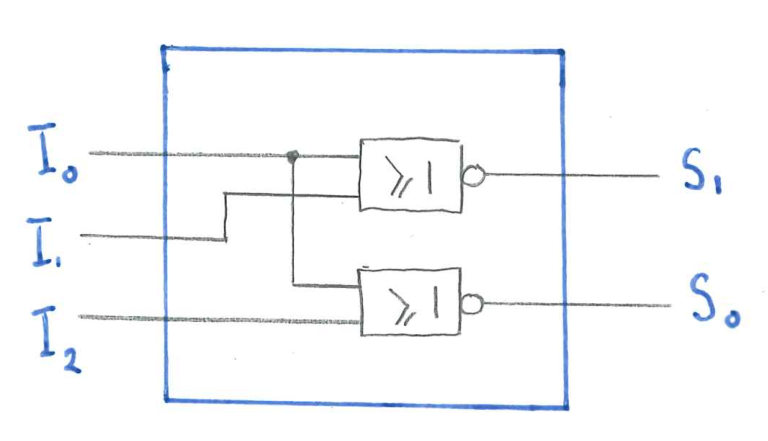
\includegraphics[width=83mm]{03_4}
          \end{center}

    \newpage

    \section{Oppgåve 5}
      Sekvenslogisk skjema for tre ulike vipper: MS-JK, positivt flanketrigga JK og
      negativt flanketrigga JK:
      \begin{center}
        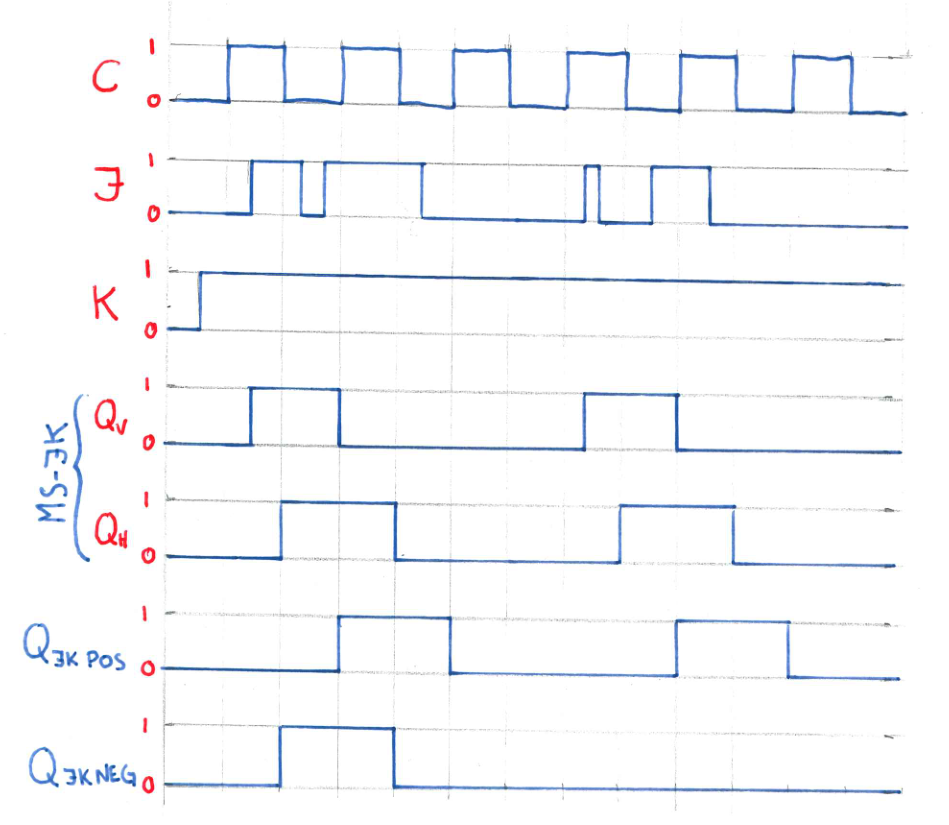
\includegraphics[width=140mm]{03_5}
      \end{center}

\end{document}
